\section{포장법}
세척이 끝난 포일이 배송 중 다시 오염 되거나 파손되는 것을 막기 위해 올바른 포장법을 적용하는 것이 중요하다. \uline{포일 포장에서 가장 신경 써야할 것은 먼지를 제거하는 것과, 포일이 구겨지지 않게 고정하는 것이다.} 포일 포장법은 제공되는 동영상을 참고할 것. 본 문서에서는 주요 사항에 대해서만 간략하게 기술한다.

포장의 외곽은 폴리카보네트 판을 이용해 물리적 지지대의 역할을 하게 한다. 압력과 SMD 저항에 의해 포일이 인접한 포일을 상하게 하는 것을 막기 위해 포일 사이에는 폼을 깔아 준다. \uline{폼의 크기는 포일이 구겨지는 것을 막기 위해 반드시 포일보다 커야한다.} 포일은 방전 필름으로 감싸 준다. 포장에 사용되는 모든 요소는 청소기와 DCR 롤러를 이용해 청소한다. 배송 중 포일이 움직이는 것과 구김이 발생하는 것을 막기 위해, 폴리카보네이트 판에 모든 요소의 네 뒤퉁이를 3M PET 테이프로 고정한다. \uline{완성된 포장팩은 청소된 비닐 봉투에 담아 외부 먼지가 유입되는 것을 막는다.} 최대 12장의 포일을 한 팩에 담을 수 있다.

\begin{figure}[htb]
  \centering
  \subfloat{
    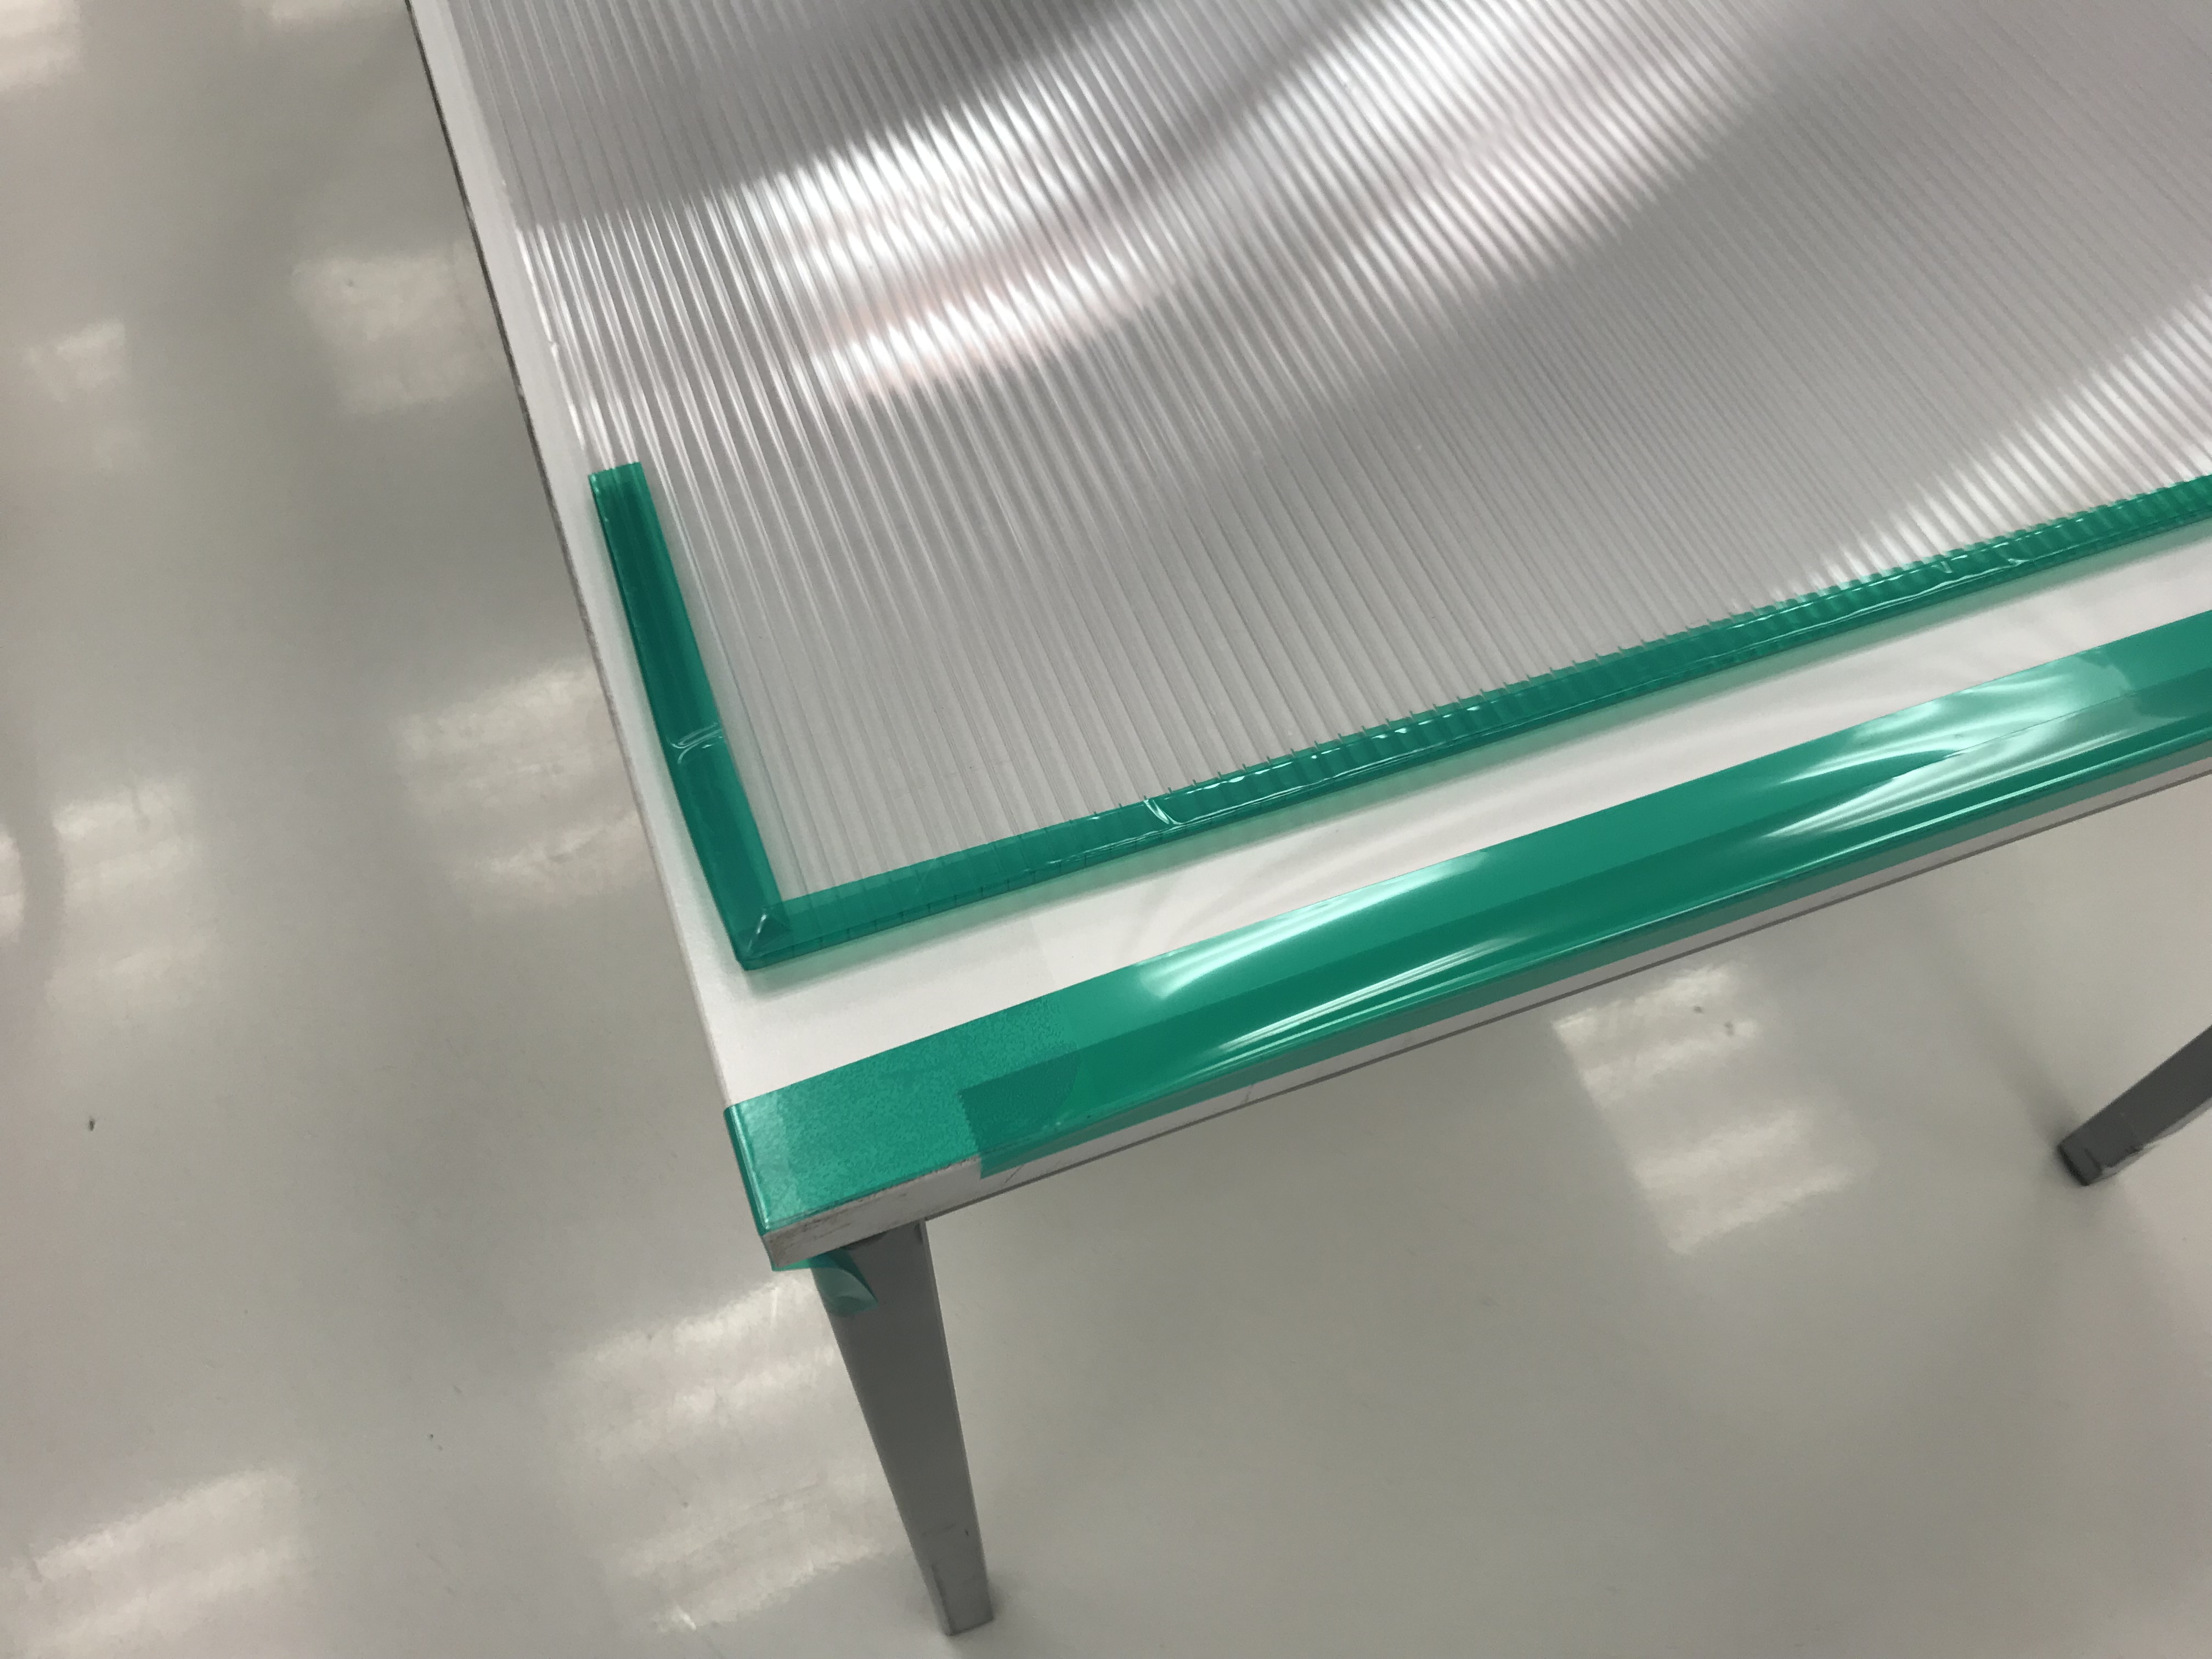
\includegraphics[width=0.40\textwidth]{PolyCarbonate.jpg}
  }
  \subfloat{
    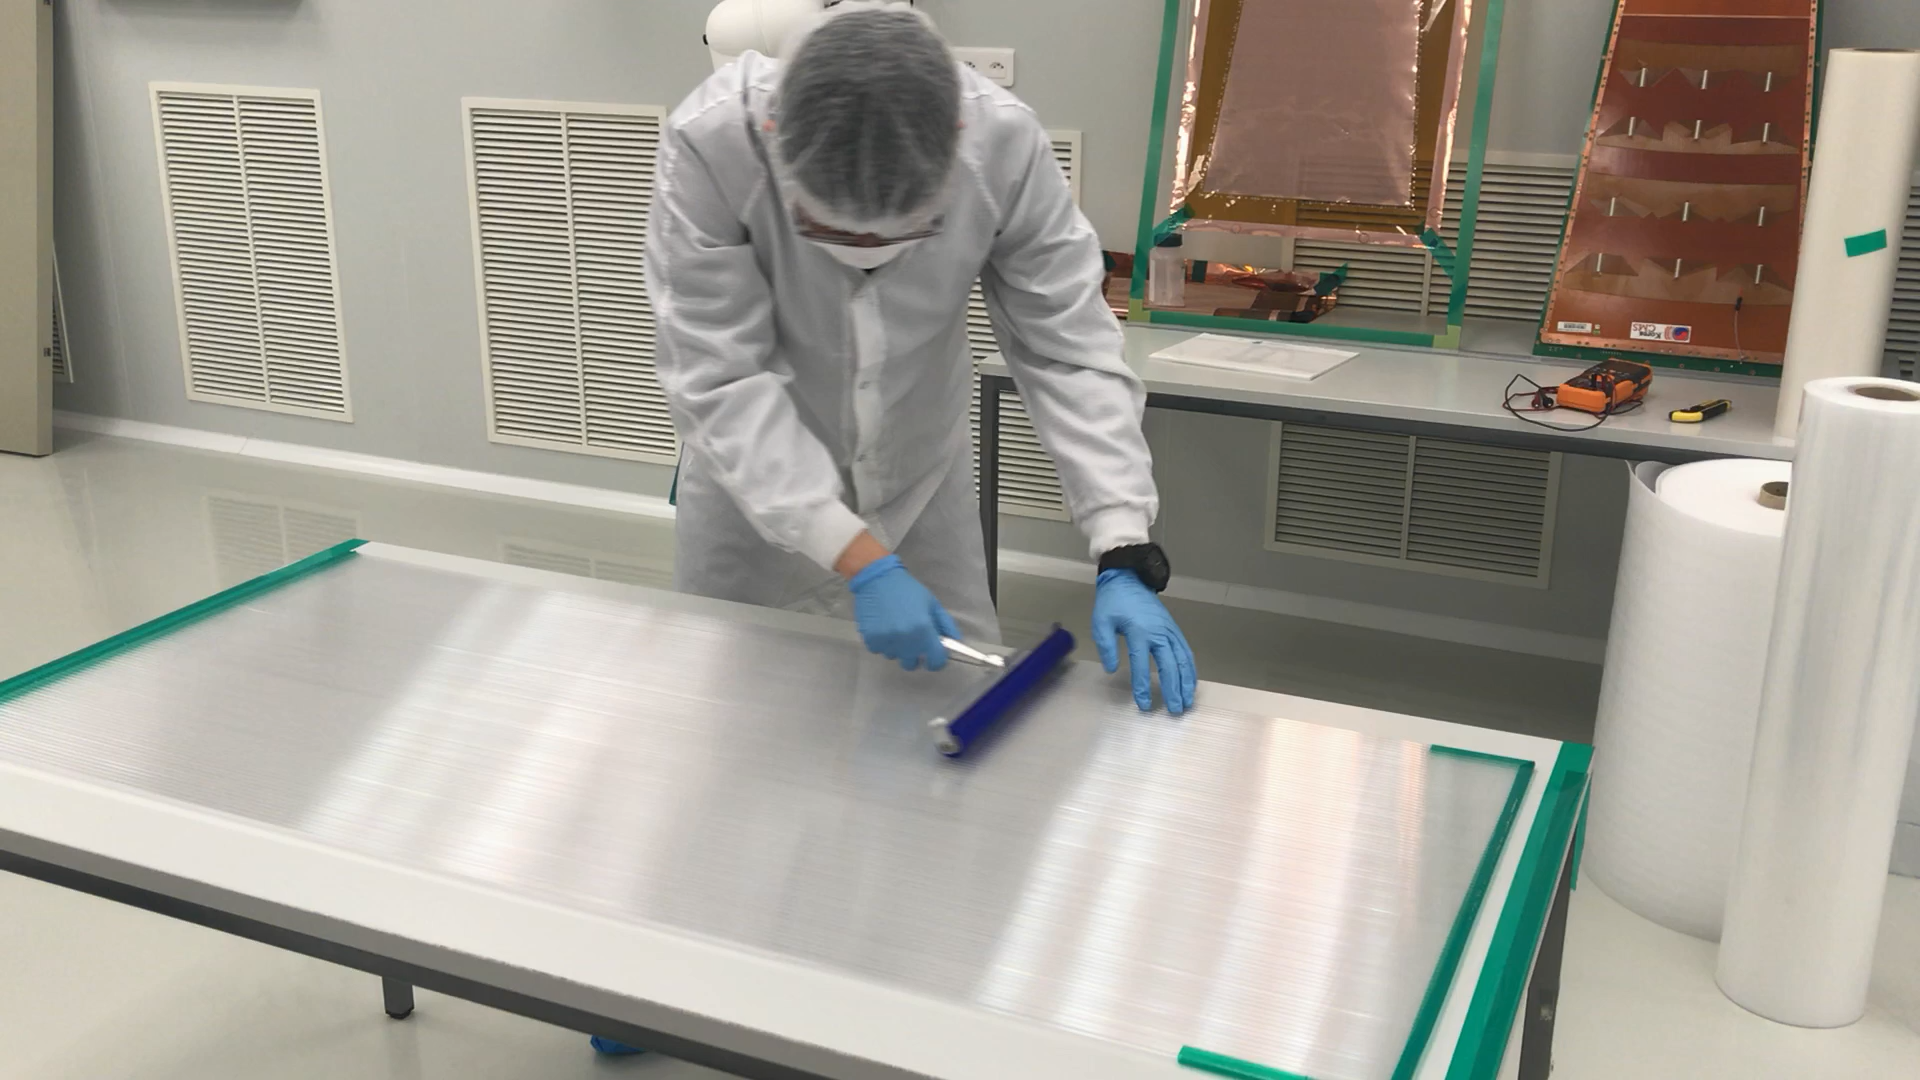
\includegraphics[width=0.40\textwidth]{Cleaning_Polycarbonate.png}
  }
  \caption[폴리카보네이트 판의 절단면 처리]{왼쪽 : 폴리카보네이트 판의 절단면은 부스러기가 나오는 것을 막기 위해 3M PET 테이프로 막아준다. 오른쪽 : 폴리카보네이트 판은 DCR 롤러로 양면을 청소한다.}
  \label{fig:polycarbonate}
\end{figure}

\begin{figure}[htb]
  \centering
  \subfloat{
    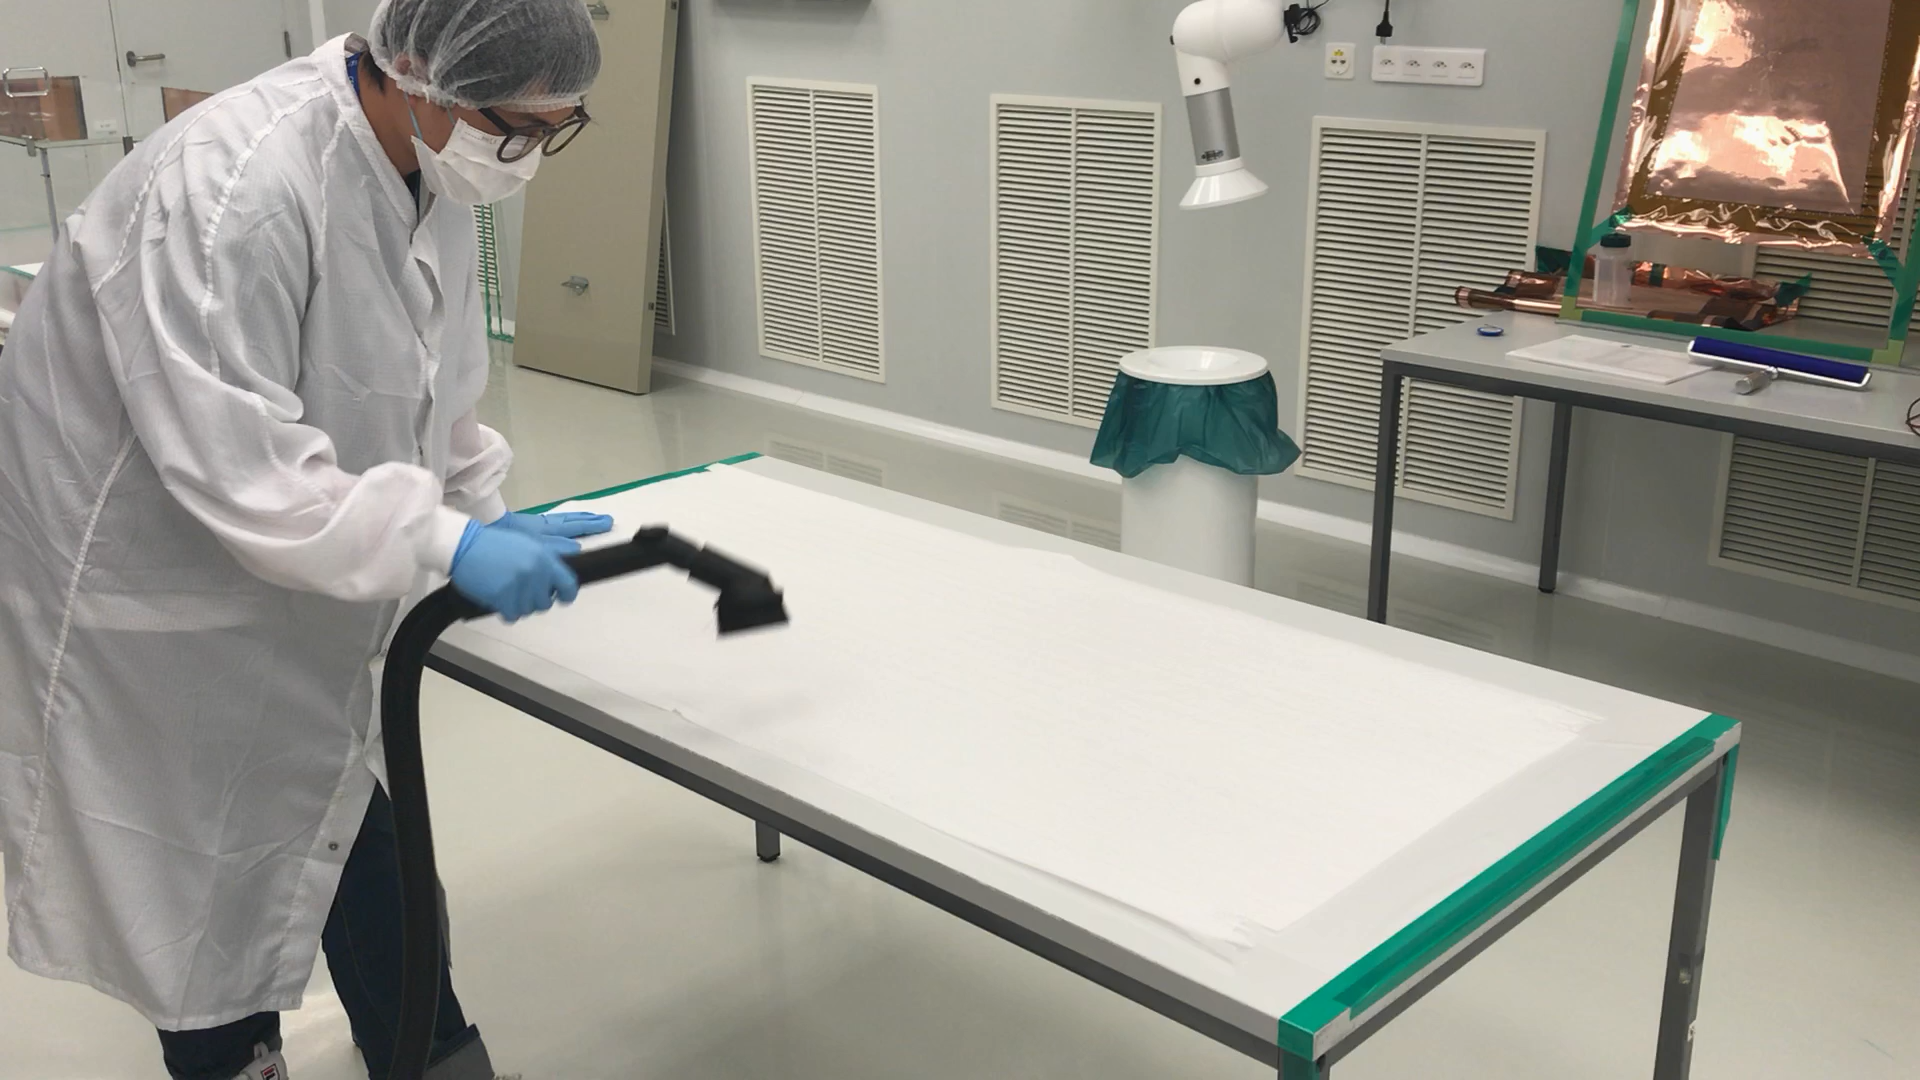
\includegraphics[width=0.40\textwidth]{cleaning_foam.png}
  }
  \subfloat{
    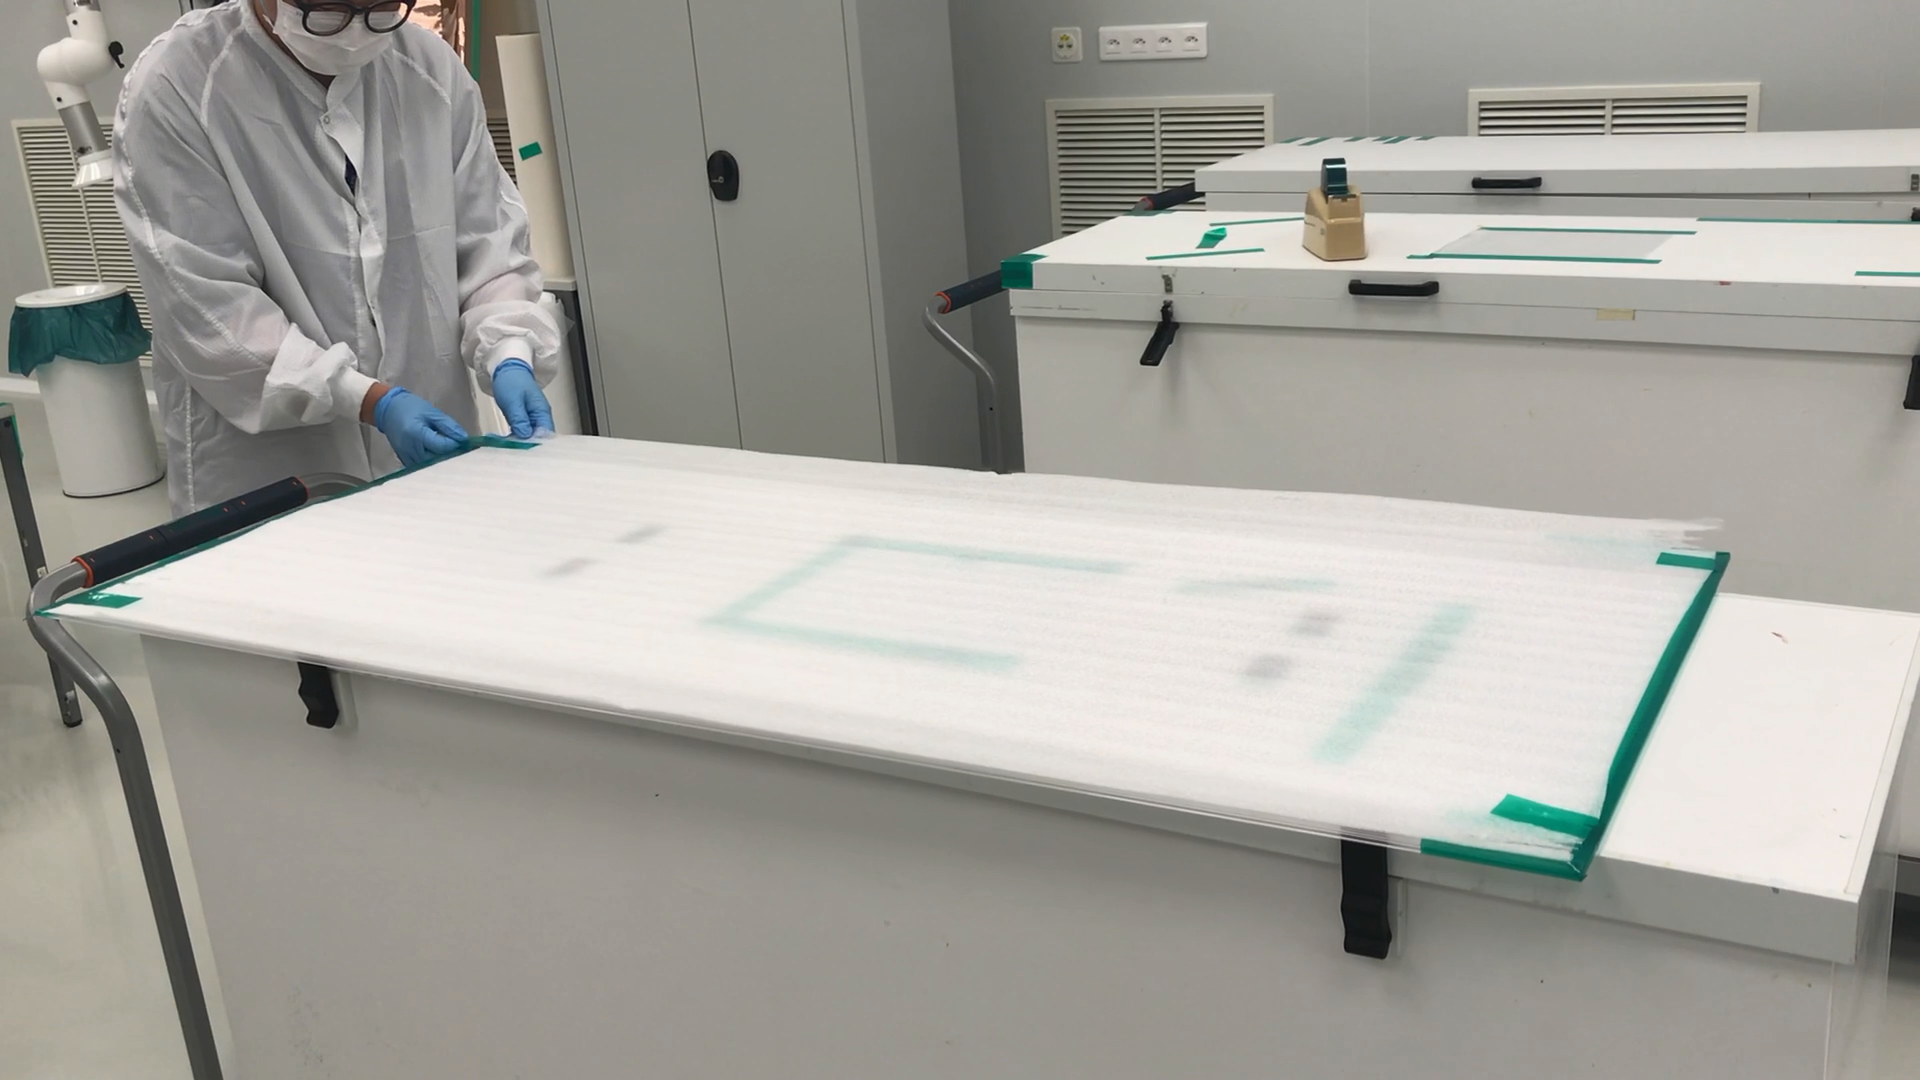
\includegraphics[width=0.40\textwidth]{fixing_foam.png}
  }
  \caption[폼의 처리]{왼쪽 : 폼은 청소기를 이용해 청소한다. \uline{폼의 크기는 포일이 구겨지는 것을 막기 위해, 최소 반드시 포일의 크기보다는 커야한다.} 오른쪽 : 폼은 폴리카보네이트 판에 3M PET 테이프로 네 뒤퉁이를 고정한다. 이 때, 구김이 없어야 한다.}
  \label{fig:foam}
\end{figure}

\begin{figure}[htb]
  \centering
  \subfloat{
    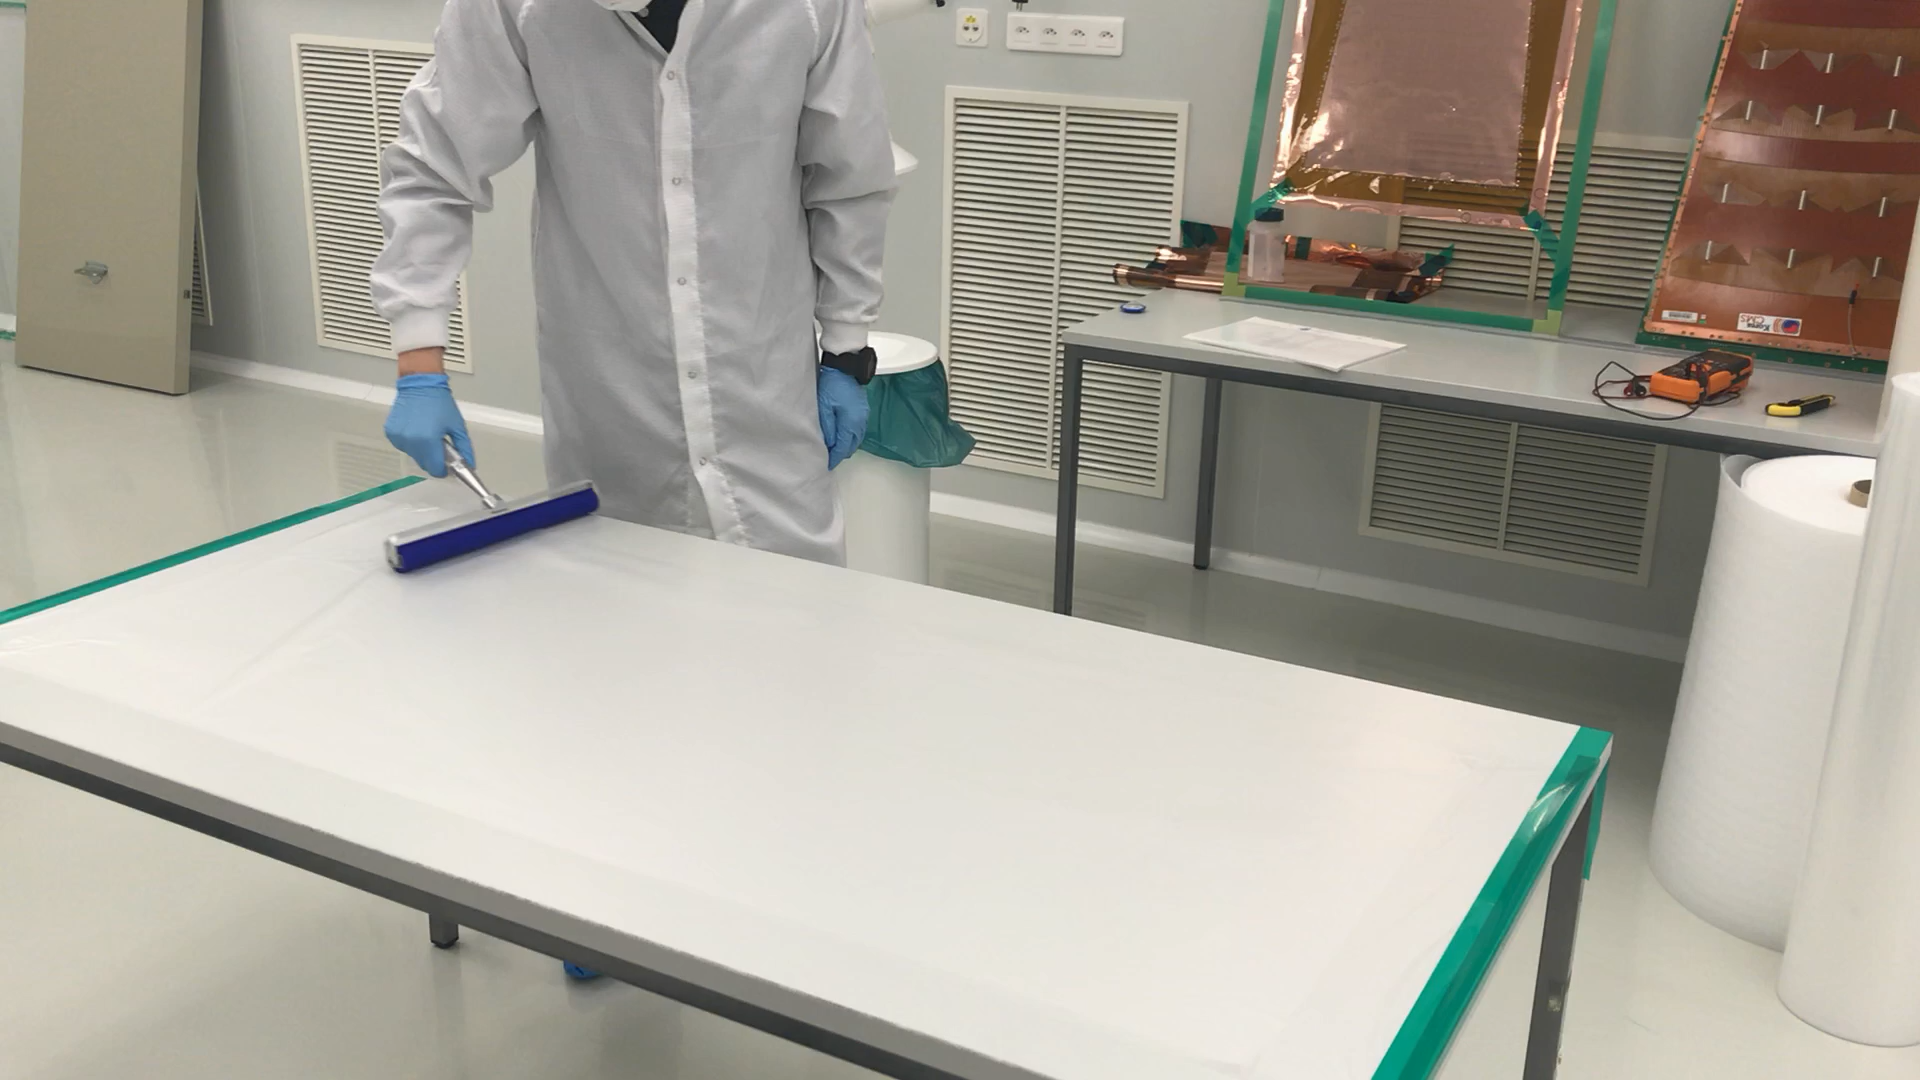
\includegraphics[width=0.40\textwidth]{cleaning_antistatic.png}
  }
  \subfloat{
    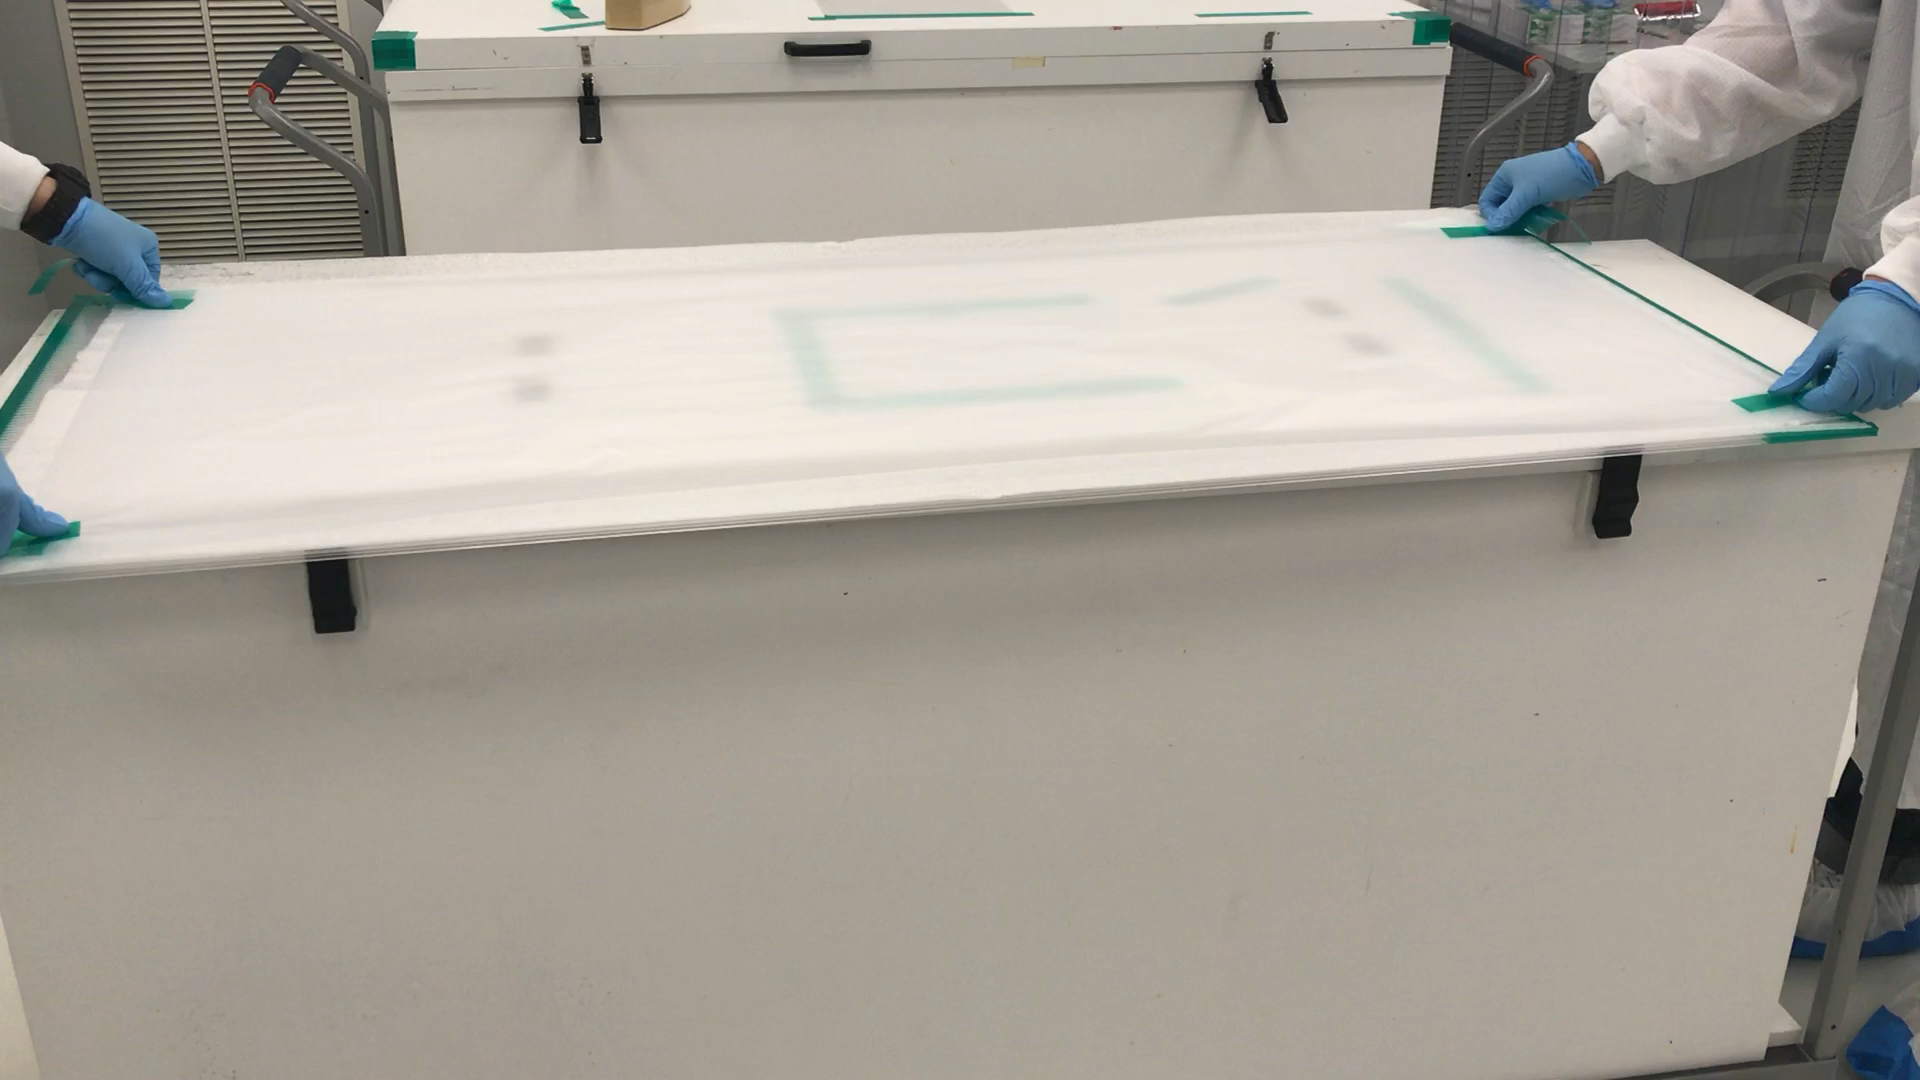
\includegraphics[width=0.40\textwidth]{fixing_antistatic.png}
  }
  \caption[방전 필름의 처리]{왼쪽 : 방전 필름은 DCR 롤러 이용해 양면을 청소한다. 오른쪽 : 방전 필름은 폴리카보네이트 판에 3M PET 테이프로 네 뒤퉁이를 고정한다. 이 때, 구김이 없어야 한다.}
  \label{fig:anti_static}
\end{figure}
\begin{figure}[htb]
  \centering
  \subfloat{
    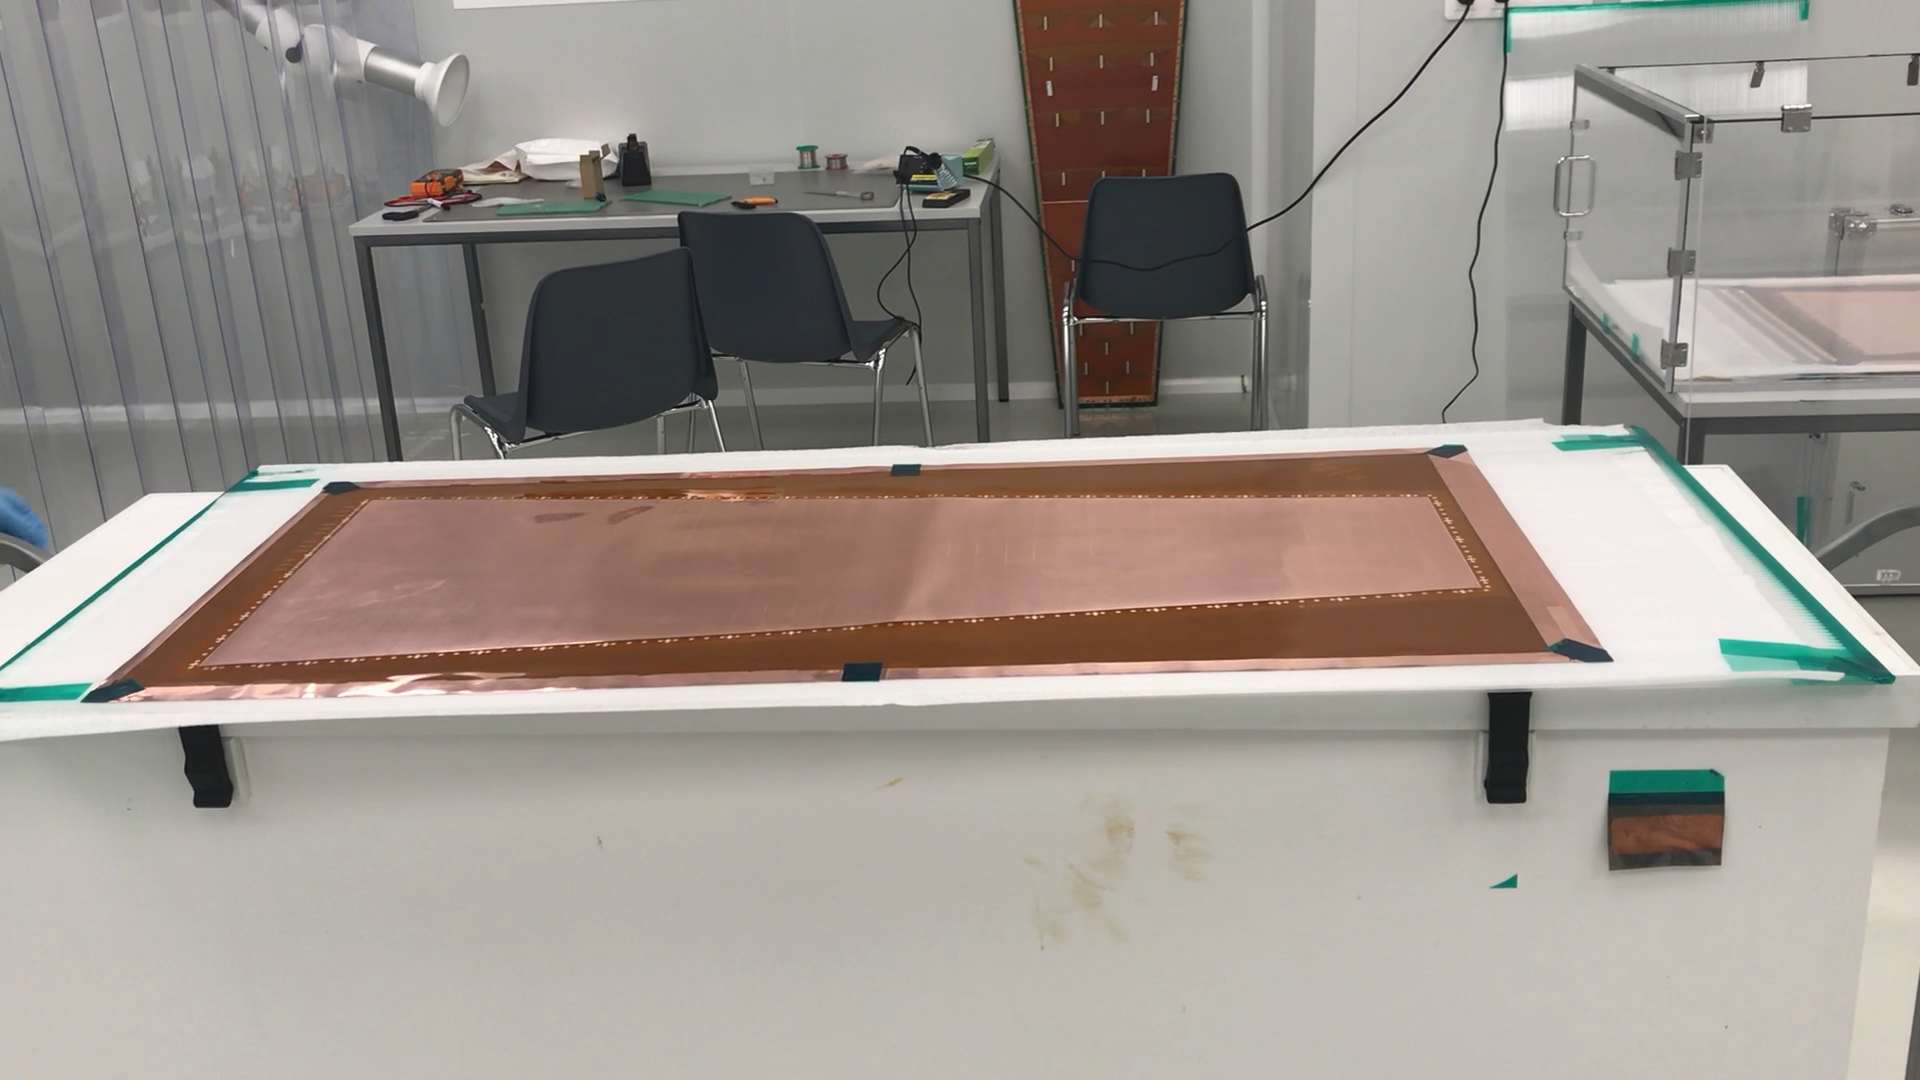
\includegraphics[width=0.40\textwidth]{fixing_foil_0.png}
  }
  \subfloat{
    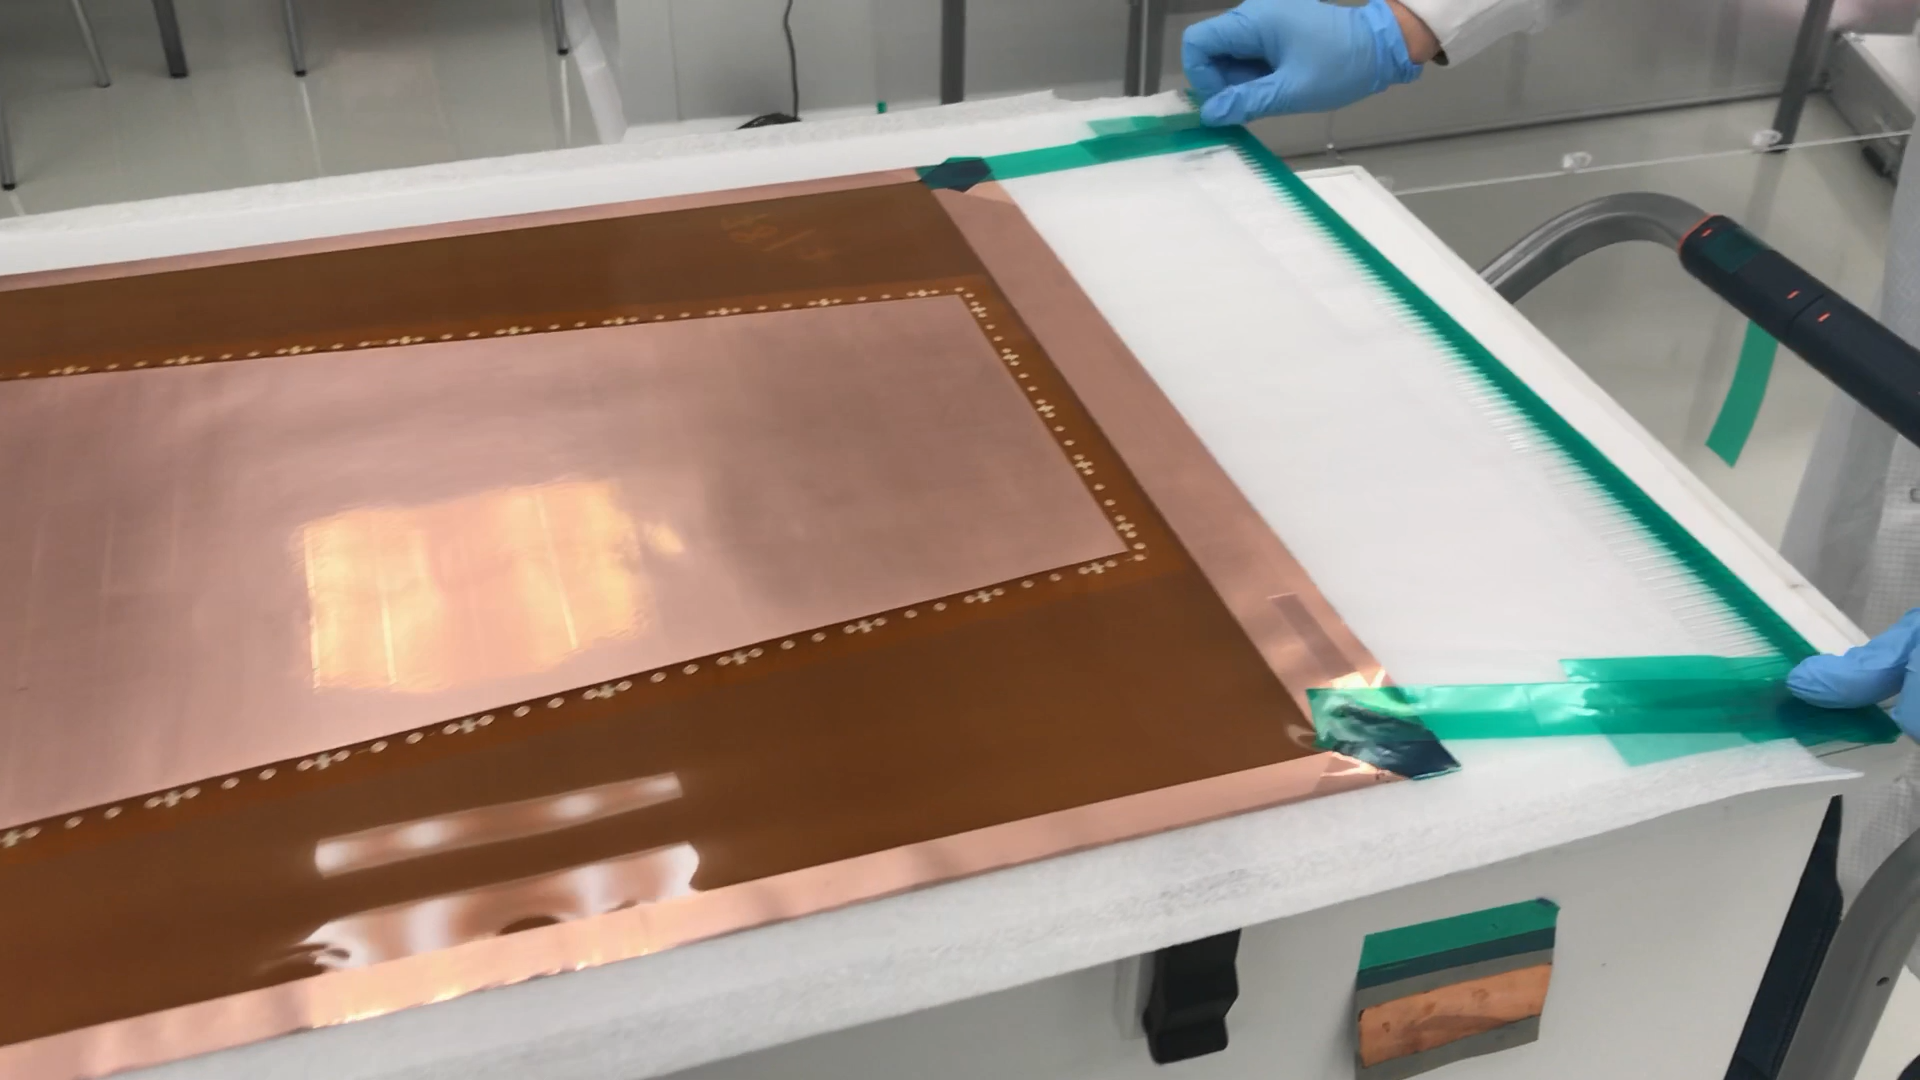
\includegraphics[width=0.40\textwidth]{fixing_foil_1.png}
  }
  \caption[GEM 포일의 고정]{왼쪽 : 포일을 고정하는 폴리카보네이트 판, 폼, 방전 필름의 크기는, GEM 포일의 구겨짐을 방지하기 위해, 포일보다 반드시 커야한다. 오른쪽: GEM 포일은 폴리카보네이트판에 3M PET 테이프로 네 뒤퉁이를 고정한다.}
  \label{fig:fixing_foil}
\end{figure}
